% Author: Izaak Neutelings (September 2021)
% Inspiration:
%   https://jila.colorado.edu/~ajsh/insidebh/penrose.html
%   https://tex.stackexchange.com/questions/99124/how-to-draw-penrose-diagrams-with-tikz
%   coordinates: https://arxiv.org/pdf/physics/0611033.pdf
%   https://arxiv.org/pdf/0711.0873.pdf
\documentclass[border=3pt,tikz]{standalone}
\usepackage{tikz}
\usepackage{amsmath} % for \text
\usepackage{mathrsfs} % for \mathscr
\usepackage{xfp} % higher precision (16 digits?)
\usepackage[outline]{contour} % glow around text
\usetikzlibrary{decorations.markings,decorations.pathmorphing}
\usetikzlibrary{angles,quotes} % for pic (angle labels)
\usetikzlibrary{arrows.meta} % for arrow size
\contourlength{1.4pt}

\newcommand{\calI}{\mathscr{I}} %\mathcal
\tikzset{>=latex} % for LaTeX arrow head
\colorlet{myred}{red!80!black}
\colorlet{myblue}{blue!80!black}
\colorlet{mygreen}{green!80!black}
\colorlet{mydarkred}{red!50!black}
\colorlet{mydarkblue}{blue!50!black}
\colorlet{mylightblue}{mydarkblue!6}
\colorlet{mypurple}{blue!40!red!80!black}
\colorlet{mydarkpurple}{blue!40!red!50!black}
\colorlet{mylightpurple}{mydarkpurple!80!red!6}
\colorlet{myorange}{orange!40!yellow!95!black}
\tikzstyle{cone}=[mydarkblue,line width=0.2,top color=blue!60!black!30,
                  bottom color=blue!60!black!50!red!30,shading angle=60,fill opacity=0.9]
\tikzstyle{cone back}=[mydarkblue,line width=0.1,dash pattern=on 1pt off 1pt]
\tikzstyle{world line}=[myblue!60,line width=0.4]
\tikzstyle{world line t}=[mypurple!60,line width=0.4]
\tikzstyle{particle}=[mygreen,line width=0.5]
\tikzstyle{photon}=[-{Latex[length=4,width=3]},myorange,line width=0.4,decorate,
                    decoration={snake,amplitude=0.9,segment length=4,post length=3.8}]
\tikzstyle{singularity}=[myred,line width=0.6,decorate,
                         decoration={zigzag,amplitude=2,segment length=6.17}]
\tikzset{declare function={%
  penrose(\x,\c)  = {\fpeval{2/pi*atan( (sqrt((1+tan(\x)^2)^2+4*\c*\c*tan(\x)^2)-1-tan(\x)^2) /(2*\c*tan(\x)^2) )}};%
  penroseu(\x,\t) = {\fpeval{atan(\x+\t)/pi+atan(\x-\t)/pi}};%
  penrosev(\x,\t) = {\fpeval{atan(\x+\t)/pi-atan(\x-\t)/pi}};%
  kruskal(\x,\c)  = {\fpeval{asin( \c*sin(2*\x) )*2/pi}};% Penrose coordinates for Kruskal
}}
\def\tick#1#2{\draw[thick] (#1) ++ (#2:0.04) --++ (#2-180:0.08)}
\def\Nsamples{20} % number samples in plot

% LIGHTCONE
\def\R{0.08} % size lightcone
\def\e{0.08} % vertical scale
\def\ang{45} % angle light cone
\def\angb{acos(sqrt(\e)*sin(\ang))} % angle ellipse center to point of tangency
\def\a{\R*sin(\ang)*sqrt(1-\e*sin(\ang)^2)/(1-\e*sin(\ang)^2)} % vertical radius
\def\b{\R*sqrt(\e)*sin(\ang)*cos(\ang)/(1-\e*sin(\ang)^2)} % horizontal radius
\def\coneback#1{ % light cone part to be drawn behind world lines
  \draw[cone back] % dashed line back
    (#1)++(-45:\R) arc({90-\angb}:{90+\angb}:{\a} and {\b});
  \draw[cone,shading angle=-60] % top edge & inside
    (#1)++(0,{\R*cos(\ang)/(1-\e*sin(\ang)^2)}) ellipse({\a} and {\b});
}
\def\conefront#1{ % light cone part to be drawn over world lines
  \draw[cone] % light cone outside
    (#1) --++ (45:\R) arc({\angb-90}:{-90-\angb}:{\a} and {\b})
     --++ (-45:2*\R) arc({90-\angb}:{-270+\angb}:{\a} and {\b}) -- cycle;
}

\begin{document}

% PENROSE DIAGRAM of Minkowski space
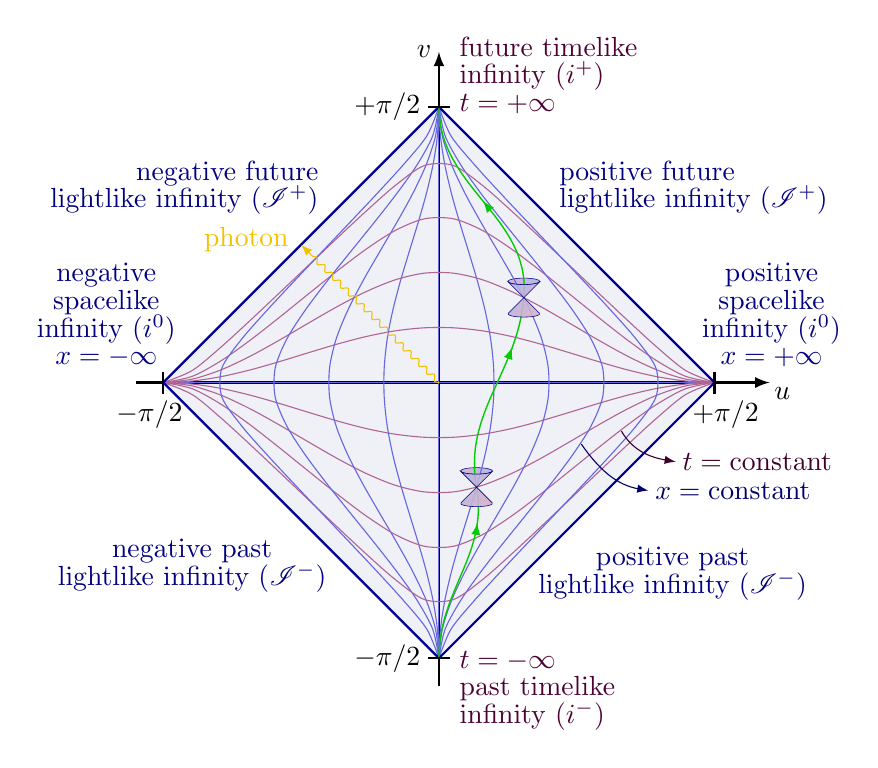
\begin{tikzpicture}[scale=3.5]
  \message{Penrose diagram^^J}
  
  \def\Nlines{4} % number of world lines (at constant r/t)
  \def\ta{tan(90*1.0/(\Nlines+1))} % constant r/t value 1
  \def\tb{tan(90*2.0/(\Nlines+1))} % constant r/t value 2
  \coordinate (O) at ( 0, 0); % center: origin (r,t) = (0,0)
  \coordinate (S) at ( 0,-1); % south: t=-infty, i-
  \coordinate (N) at ( 0, 1); % north: t=+infty, i+
  \coordinate (W) at (-1, 0); % east:  r=-infty, i0
  \coordinate (E) at ( 1, 0); % west:  r=+infty, i0
  \coordinate (X) at ({penroseu(\tb,\tb)},{penrosev(\tb,\tb)});
  \coordinate (X0) at ({penroseu(\ta,-\tb)},{penrosev(\ta,-\tb)});
  
  % AXES
  \fill[mylightblue] (N) -- (E) -- (S) -- (W) -- cycle;
  \draw[->,thick] (-1.1,0) -- (1.2,0) node[below right=-2] {$u$};
  \draw[->,thick] (0,-1.1) -- (0,1.2) node[left=-1] {$v$};
  
  % INFINITY LABELS
  \node[right=6,above left=-2,mydarkblue,align=center] at (-1,0.04)
    {negative\\[-2]spacelike\\[-2]infinity ($i^0$)\\[-2]$x=-\infty$};
  \node[left=6,above right=-2,mydarkblue,align=center] at (1,0.04)
    {positive\\[-2]spacelike\\[-2]infinity ($i^0$)\\[-2]$x=+\infty$};
  \node[above=6,below right=0,mydarkpurple,align=left] at (0.04,-1)
    {$t=-\infty$\\[-2]past timelike\\[-2]infinity ($i^-$)};
  \node[below=6,above right=0,mydarkpurple,align=left] at (0.04,1)
    {future timelike\\[-2]infinity ($i^+$)\\[-2]$t=+\infty$};
  \node[mydarkblue,above right,align=left] at (55:0.7)
    {positive future\\[-2]lightlike infinity ($\calI^+$)};
  \node[mydarkblue,below right,align=center] at (-60:0.65)
    {positive past\\[-2]lightlike infinity ($\calI^-$)};
  \node[mydarkblue,above left,align=right] at (125:0.7)
    {negative future\\[-2]lightlike infinity ($\calI^+$)};
  \node[mydarkblue,below left,align=center] at (-125:0.65)
    {negative past\\[-2]lightlike infinity ($\calI^-$)};
  
  % CONE BACK
  \coneback{X};
  \coneback{X0};
  
  % WORLD LINES
  \draw[world line] (N) -- (S);
  \draw[world line] (W) -- (E);
  \message{Making world lines...^^J}
  \foreach \i [evaluate={\c=\i/(\Nlines+1); \ct=tan(90*\c);}] in {1,...,\Nlines}{
    \message{  Running i/N=\i/\Nlines, c=\c, tan(90*\c)=\ct...^^J}
    \draw[world line t,samples=\Nsamples,smooth,variable=\t,domain=-1:1] % constant t
      plot(\t,{-penrose(\t*pi/2,\ct)})
      plot(\t,{ penrose(\t*pi/2,\ct)});
    \draw[world line,samples=\Nsamples,smooth,variable=\x,domain=-1:1] % constant r
      plot({-penrose(\x*pi/2,\ct)},\x)
      plot({ penrose(\x*pi/2,\ct)},\x);
  }
  \draw[thick,blue!60!black] (N) -- (E) -- (S) -- (W) -- cycle;
  
  % CONSTANT
  \draw[->,mydarkpurple!80!black,shorten <=0.4] % constant r
    (0.66,{-penrose(0.66*pi/2,tan(90*3/(\Nlines+1)))}) to[out=-60,in=170]++ (-30:0.23)
    node[right=-1] {$t=\text{constant}$};
  \draw[->,mydarkblue!80!black,shorten <=0.4] % constant t
    ({penrose(-0.22*pi/2,tan(90*3/(\Nlines+1)))},-0.22) to[out=-55,in=170]++ (-35:0.3)
    node[right=-1] {$x=\text{constant}$};
  
  % PARTICLE
  \draw[particle,decoration={markings,mark=at position 0.24 with {\arrow{latex}},
                                      mark=at position 0.55 with {\arrow{latex}},
                                      mark=at position 0.82 with {\arrow{latex}}},postaction={decorate}]
    (S) to[out=90,in=-80] (X0) to[out=100,in=-95] (X) to[out=85,in=-90] (N);
  
  % LIGHT CONE FRONT
  \conefront{X};
  \conefront{X0};
  
  % PHOTON
  \draw[->,photon] (O) -- (-0.5,0.5) node[above=2,left=1] {photon};
  
  % TICKS
  \tick{W}{90} node[left=5,below=-1] {$-\pi/2$};
  \tick{E}{90} node[right=4,below=-1] {$+\pi/2$};
  \tick{S}{ 0} node[left=-1] {$-\pi/2$};
  \tick{N}{ 0} node[left=-1] {$+\pi/2$};
  
\end{tikzpicture}



\end{document}  